\section{Eulertouren und Hamiltonkreise}
\subsubsection{Eulertouren}
Euler (1736): Königsberger Brückenproblem: \\
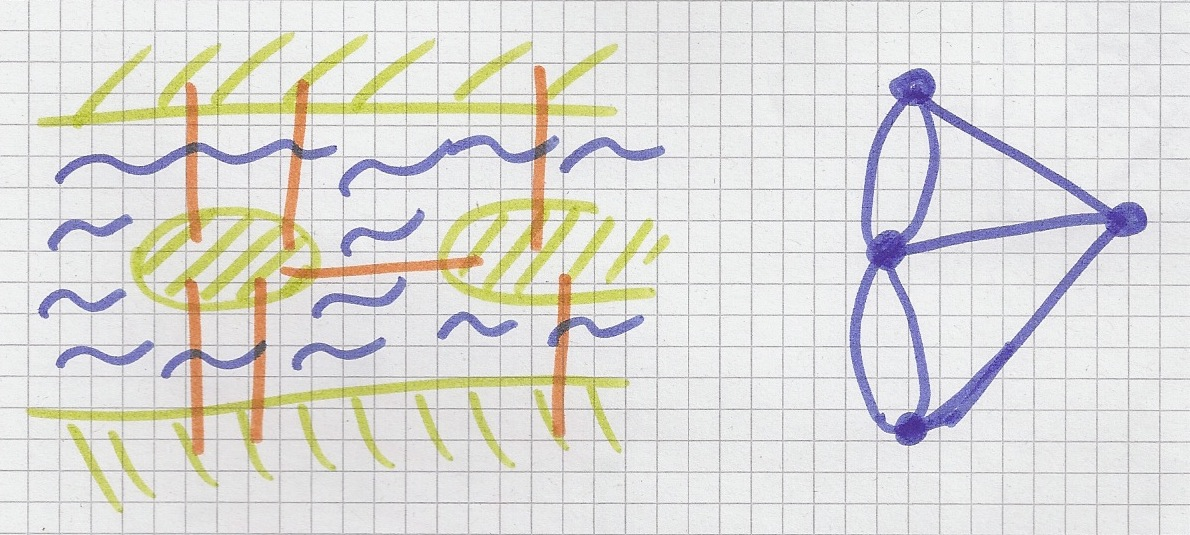
\includegraphics[width=\textwidth]{Bild49} \\
Gibt es einen Weg, der jede Brücke genau einmal benützt? \\
\begin{def*}[note = Eulertour (ET) , index = Eulertour]
	\text{Geschlossener} (Anfang = Ende) Kantenzug, der \textbf{jede Kante} genau einmal enthält.
\end{def*}
Gibt es Eulertour im gegebenen Graphen? Nein. \\
\begin{satz*}[note = (Euler)]
	Ein zusammenhängender Graph (oder Multi-Graph) hat \textbf{genau dann} eine Eulertour, wenn alle Knotengrade gerade sind.\\
	\begin{bew}
		Bedingung notwendig: Jeder Knoten wird gleich oft erreicht und verlassen. \\
		Bedingung hinreichend: Konstruktiv: Zufälliger Knoten $\rightarrow v_1$, jeweils zufällige unbenützte Kante $\rightarrow\rightarrow\rightarrow v_1$. Falls es noch unbenutzte Kanten gibt, dann auch solche, die an $W_1$ grenzen. Analog $W_2$. $\rightarrow W$ geschlossen. Prozess iterieren. Muss abbrechen $(\abs{E} < \infty) \rightarrow$ Eulertour. $\blacksquare$
	\end{bew}
	Wir haben zusätzlich bewiesen: Eine Eulertour kann in linearer Zeit $\sim \abs{E}$ gefunden werden.
\end{satz*}
\begin{bsp*}
	$K_n$ hat ET $\iff$ $n$ ist ungerade. \\
	$Q_d$ hat ET $\iff$ $d$ ist gerade. \\
	Baum $B$ hat keine ET (ausser $\cdot$ )
\end{bsp*}

\subsubsection{Hamiltonkreise}
\begin{def*}[note = Hamiltonkreis (HK) , index = Hamiltonkreis]
	\textbf{Kreis}, der jeden Knoten genau einmal besucht. Ein Graph, der einen HK hat, heisst \text{hamiltonisch}.
\end{def*}
\begin{bsp*}
	hamiltonisch:\\
	$C_k$ \\
	Rad \\
	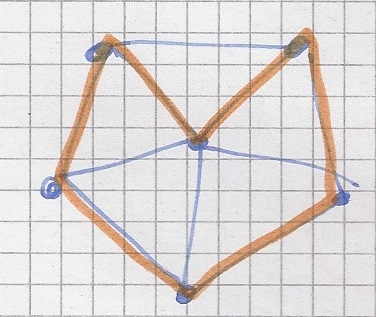
\includegraphics{Bild50} \\
	nicht hamiltonisch: \\
	Stern \\
	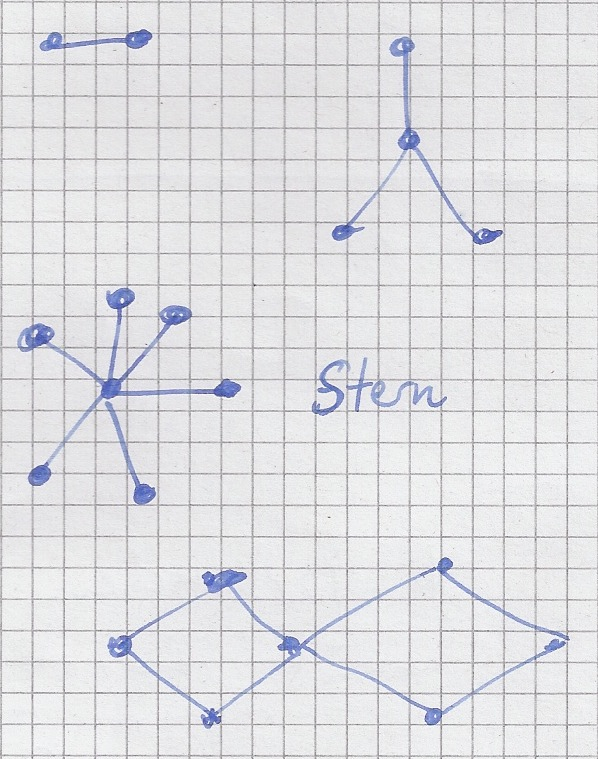
\includegraphics{Bild51} \\
	Bäume
\end{bsp*}
Wann ist $M_{m,n}$ hamiltonisch?\\
\begin{tabular}{lll}
	$M_{1,2}$:	&nicht	&hamiltonisch	\\
	$M_{2,2}$:	&		&hamilotnisch	\\
	$M_{2,3}$:	&		&hamiltonisch	\\
	$M_{3,3}$:	&nicht	&hamiltonisch, da nicht gleich viele gelbe und grüne
\end{tabular}\\
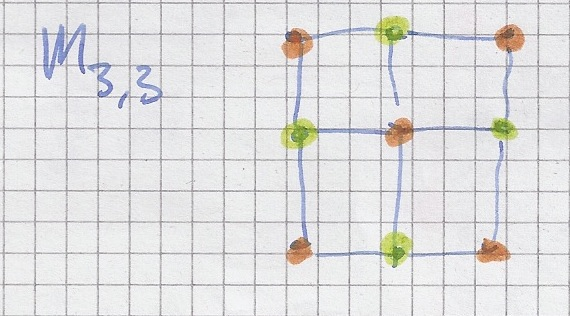
\includegraphics{Bild52} \\
Also: $M_1,n$ nicht hamiltonisch. \\
$m,n \geq 2 : M_{m,n}$ hamiltonisch $\iff m \cdot n = \abs{V}$ gerade \\
\begin{bew}
	$m$ gerade\\
	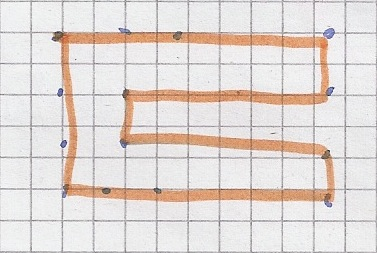
\includegraphics{Bild53}
\end{bew}
Wann ist $Q_d$ hamiltonisch?\\
\begin{tabular}{lll}
	$d=0$:	&nicht	&hamiltonisch	\\
	$d=1$:	&nicht	&hamiltonisch	\\
	$d=2$:	&		&hamiltonisch	\\
	$d=3$:	&		&hamiltonisch	\\
	$d=4$:	&		&hamiltonisch	
\end{tabular}\\
$Q_d$ist hamiltonisch für alle $d \geq 2$.\\
\begin{bew}
	BILD \\
	Induktion über $d$ \\
	Verankerung: $d=2$. \\
	Induktionsschritt: $d \rightarrow d + 1$\\
	IV: $Q_d$ hat HK C. \\
	$C$ und $C'$ enthalten alle Knoten.\\
	Entferne Kanten $(a0,b0)$ und $(a1,b1)$ und fügen $(a0,a1)$ und $(b0,b1)$ ein. $\blacksquare$
\end{bew}
Entscheiden ob ein Graph hamiltonisch ist NP-vollständig. \\
\begin{tabular}{lcl}
	Euler		&$\hat{=}$	&Tautologieproblem KNF	\\
	Hamilton	&$\hat{=}$	&Erfüllbarkeitsproblem DNF	
\end{tabular}\\
\begin{satz*}
	$G=(V,E)$ mit $\deg(v) \geq \frac{\abs{V}}{2}, \abs{V} \geq 4$ für alle $v \implies G$ hamiltonisch. \\
	\begin{bew}
		Indirekt: Gegenbsp. mit max. $\abs{E}$ (für best. $\abs{V}$) \\
		Es gibt $\{ u,v \} \notin E$. ($G$ vollständig $\implies G$ hamiltonisch) \\
		$G' = (V,E \cup \{\{ u,v \}\})$ hat HK (Maximalität von $\abs{E}$) \\
		HK muss $\{ u,v \}$ enthalten (sonst hätte $G$ einen HK) \\
		$\abs{V} = n$ \\
		BILD \\
	\end{bew}
\end{satz*}
	